% TikZ schematic: Filter Taxonomy (standalone compile)
\documentclass[tikz,border=10pt]{standalone}
\usepackage{tikz}
\usetikzlibrary{positioning,arrows.meta}

\begin{document}
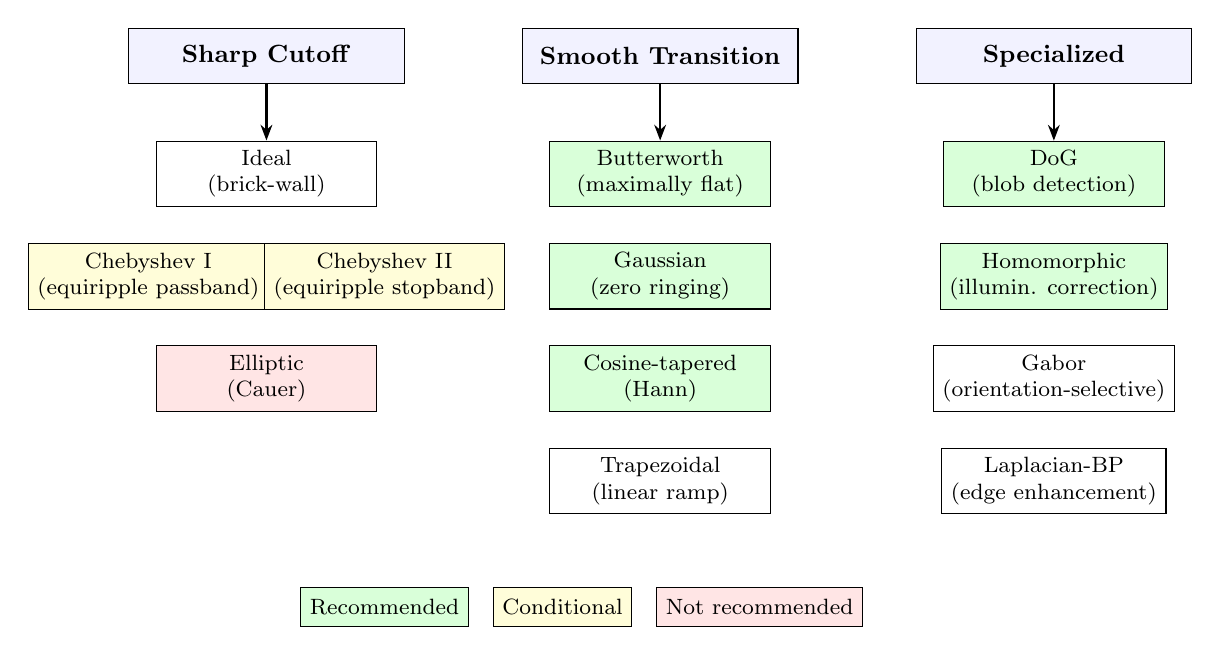
\begin{tikzpicture}[
    node distance=0.8cm and 1.5cm,
    cat/.style={rectangle, draw, fill=blue!5, minimum width=3.5cm, minimum height=0.7cm, align=center, font=\small},
    filt/.style={rectangle, draw, fill=white, minimum width=2.8cm, minimum height=0.6cm, align=center, font=\footnotesize},
    rec/.style={rectangle, draw, fill=green!15, minimum width=2.8cm, minimum height=0.6cm, align=center, font=\footnotesize},
    warn/.style={rectangle, draw, fill=yellow!15, minimum width=2.8cm, minimum height=0.6cm, align=center, font=\footnotesize},
    bad/.style={rectangle, draw, fill=red!10, minimum width=2.8cm, minimum height=0.6cm, align=center, font=\footnotesize},
    arrow/.style={-{Stealth[length=2mm]}, thick}
]

% Categories
\node[cat] (sharp) at (0,4) {\textbf{Sharp Cutoff}};
\node[cat] (smooth) at (5,4) {\textbf{Smooth Transition}};
\node[cat] (special) at (10,4) {\textbf{Specialized}};

% Sharp cutoff filters
\node[filt] (ideal) at (0,2.5) {Ideal\\(brick-wall)};
\node[warn] (cheb1) at (-1.5,1.2) {Chebyshev I\\(equiripple passband)};
\node[warn] (cheb2) at (1.5,1.2) {Chebyshev II\\(equiripple stopband)};
\node[bad] (elliptic) at (0,-0.1) {Elliptic\\(Cauer)};

% Smooth transition filters
\node[rec] (butter) at (5,2.5) {Butterworth\\(maximally flat)};
\node[rec] (gauss) at (5,1.2) {Gaussian\\(zero ringing)};
\node[rec] (cosine) at (5,-0.1) {Cosine-tapered\\(Hann)};
\node[filt] (trap) at (5,-1.4) {Trapezoidal\\(linear ramp)};

% Specialized filters
\node[rec] (dog) at (10,2.5) {DoG\\(blob detection)};
\node[rec] (homo) at (10,1.2) {Homomorphic\\(illumin. correction)};
\node[filt] (gabor) at (10,-0.1) {Gabor\\(orientation-selective)};
\node[filt] (lapl) at (10,-1.4) {Laplacian-BP\\(edge enhancement)};

% Arrows from categories
\draw[arrow] (sharp) -- (ideal);
\draw[arrow] (smooth) -- (butter);
\draw[arrow] (special) -- (dog);

% Legend
\node[draw, fill=green!15, minimum width=1.5cm, minimum height=0.5cm, font=\footnotesize] (leg1) at (1.5,-3) {Recommended};
\node[draw, fill=yellow!15, minimum width=1.5cm, minimum height=0.5cm, font=\footnotesize, right=0.3cm of leg1] (leg2) {Conditional};
\node[draw, fill=red!10, minimum width=1.5cm, minimum height=0.5cm, font=\footnotesize, right=0.3cm of leg2] (leg3) {Not recommended};

\end{tikzpicture}
\end{document}
